\documentclass[10pt]{article}
\usepackage[OE]{express}

\begin{document}
\title{Polarized Illumination For Determining Single-Molecule Orientation:
  Modeling and Instrument Design}

\author{Talon Chandler,\authormark{1} Author Two,\authormark{2,*} and Author Three\authormark{2,3}}

\address{\authormark{1}Peer Review, Publications Department, The Optical Society, 2010 Massachusetts Avenue NW, Washington, DC 20036, USA\\
\authormark{2}Publications Department, The Optical Society, 2010 Massachusetts Avenue NW, Washington, DC 20036, USA\\
\authormark{3}Currently with the Department of Electronic Journals, The Optical Society, 2010 Massachusetts Avenue NW, Washington, DC 20036, USA}

\email{talonchandler@talonchandler.com} %% email address is required

%%%%%%%%%%%%%%%%%%% abstract and OCIS codes %%%%%%%%%%%%%%%%
\begin{abstract*}
Abstract here. 
\end{abstract*}

\ocis{(180.0180) Microscopy; (260.5430) Polarization; (110.0110) Imaging systems; (180.2520) Fluorescence microscopy; (180.6900) Three-dimensional microscopy.}  

%%%%%%%%%%%%%%%%%%%%%%% References %%%%%%%%%%%%%%%%%%%%%%%%%
\begin{thebibliography}{99}
\bibitem{gallo99} K. Gallo and G. Assanto, ``All-optical diode based on second-harmonic generation in an asymmetric waveguide,'' \josab {\bfseries 16}(2), 267--269 (1999).
\end{thebibliography}

\section{Introduction}
Single molecule orientation determination is important because

A variety of techniques have been tested to determine the orientation of
single molecules:

polarized detection [Fourkas], shape analysis [Moerner], other things from
Moerner review. 

We propose polarized illumination as an complementary method to polarized
detection. We get the speed (no shape analysis required).

In this work we make three contributions:
\begin{itemize}
\item we develop the polarized illumination forward model for a broad class of
  microscopes (section 2.X-2.X)
\item we develop metrics to compare the performance of polarized illumination
  microscopes 
\item we use these metrics to compare microscopes design and make recommendations
  for polarized illumination microscopes. 
\end{itemize}


\section{Methods}
\subsection{Illumination Model}

\subsection{Detection Model}

\subsection{Complete Forward Model}
\begin{align}
  I = I_{\text{tot}}\eta_{\text{exc}}\eta_{\text{det}}
\end{align}

\subsection{Microscope Designs}

\subsection{Evaluation Metrics}
\begin{align}
  F &= \sum_{i=0}^N \frac{1}{I}
  \begin{bmatrix}
    \frac{\partial^2 I}{\partial \Theta^2}&\frac{\partial I}{\partial \Theta}\frac{\partial I}{\partial \Phi}\\
    \frac{\partial I}{\partial \Theta}\frac{\partial I}{\partial \Phi}&\frac{\partial^2 I}{\partial \Phi^2}\\    
  \end{bmatrix}\\
  \sigma_{\Omega} &= \frac{\sin\Theta}{\sqrt{\text{det}\{F\}}}
\end{align}
We call $\sigma_{\Omega}$ the \emph{solid-angle uncertainty}. 
We sampled $\sigma_{\Omega}$ on 100,000 approximately equally
spaced points on the unit sphere and calculated the \emph{coefficient of variation}
$c_v$ of these points where
\begin{align}
  c_v = \frac{\sigma_{\sigma_{\Omega}}}{\mu_{\sigma_{\Omega}}}
\end{align}

\section{Results}
\subsection{One-Arm Designs}
\begin{figure}[htbp]
\centering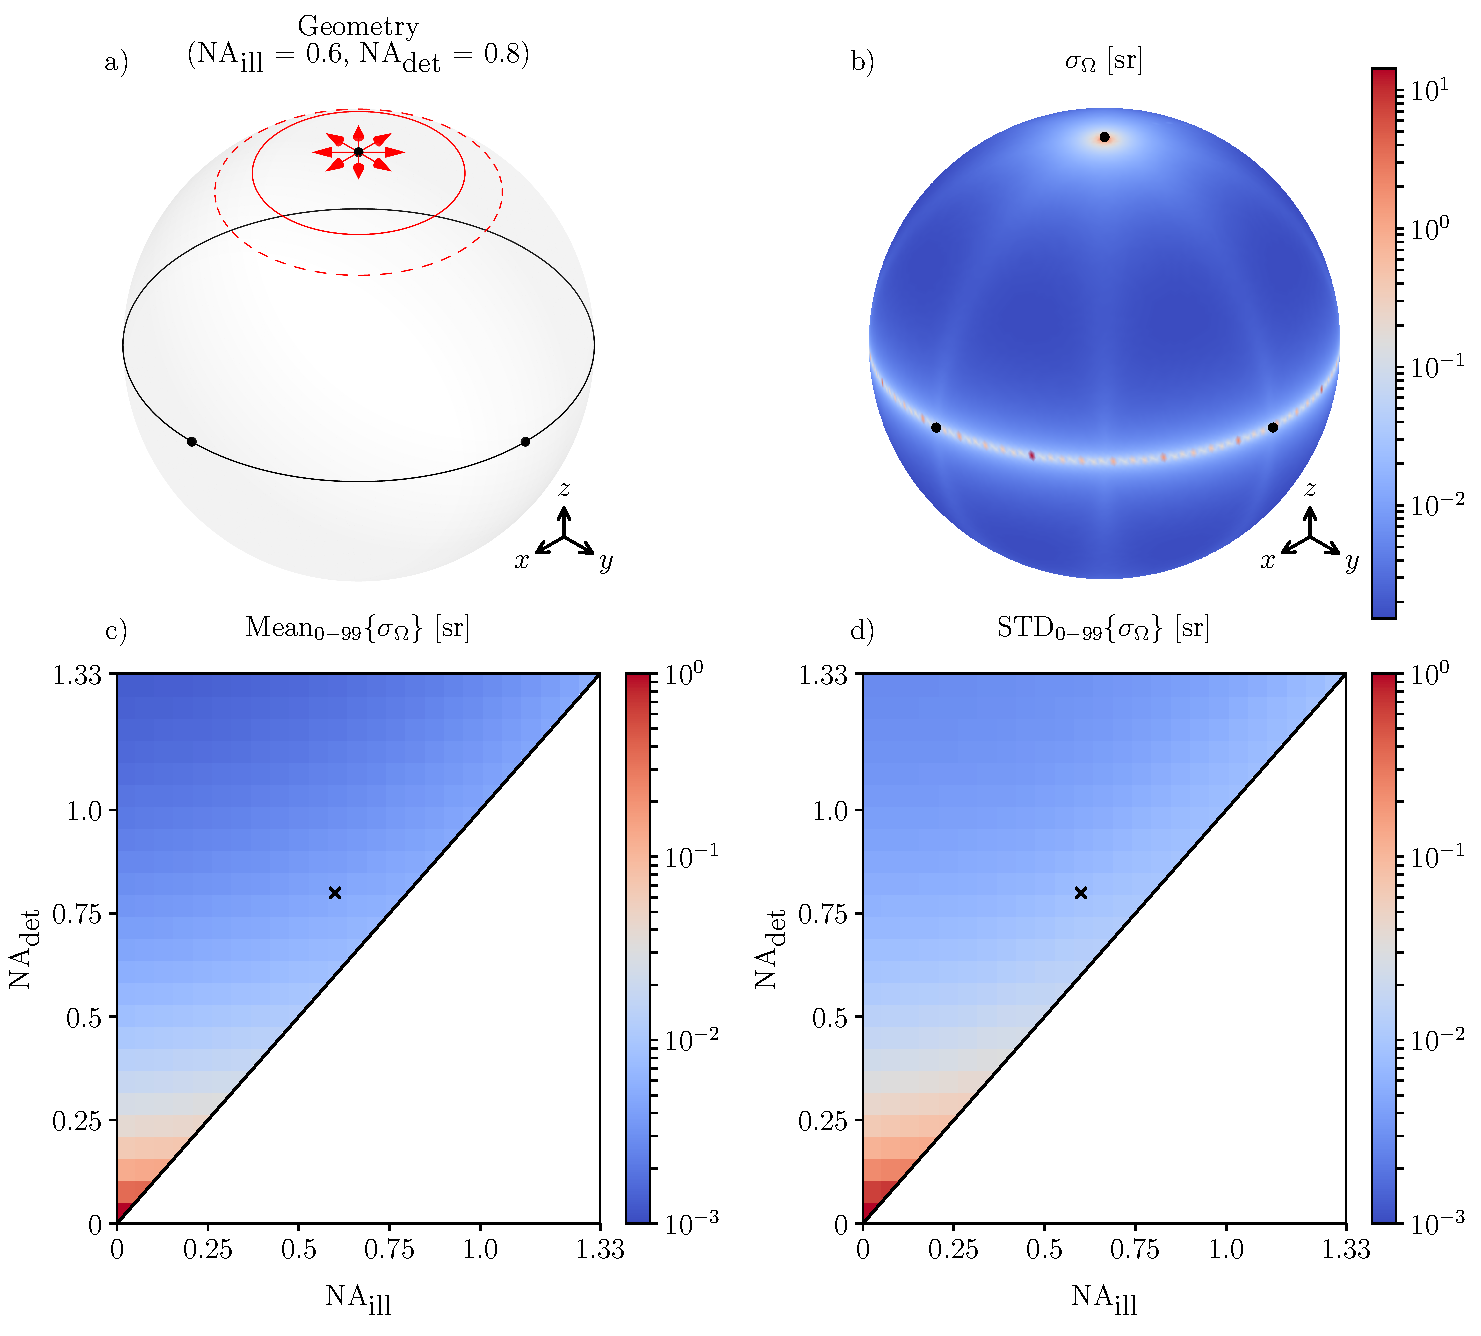
\includegraphics[width=\textwidth]{single-arm}
\caption{\textbf{Left:} Schematic of a single-arm four-frame epi-illumination
  microscope with NA = 0.8 and $n = 1.33$. The solid and dashed lines enclose
  the illumination and detection solid angles, respectively, and the arrows
  indicate the illumination polarization orientations. \textbf{Right:} Solid
  angle uncertainty for the same microscope when $I_{\text{tot}} = 1000$
  photons. Note the regions of high uncertainty near the equator and poles
  as noted in XXX.}
\end{figure}

\subsection{Two-Arm Designs}
\subsection{Three-Arm Designs}

\section{Discussion}

\section{Conclusion}

\section*{Funding}
TODO

\section*{Acknowledgments}
TODO

\section*{Disclosures}
The authors declare that there are no conflicts of interest related to this article.

\end{document}
